\documentclass[12pt]{article}

\usepackage[brazilian]{babel}
\usepackage[utf8]{inputenc}
\usepackage[T1]{fontenc}
\usepackage{graphicx}
\usepackage{geometry}
\usepackage{booktabs}
\usepackage{float}
\usepackage{longtable}
\usepackage[table]{xcolor}
\usepackage{tcolorbox}
\usepackage{enumitem}
\usepackage{pdflscape}
\usepackage{hyperref}

\geometry{a4paper, left=3cm, top=3cm, right=2cm, bottom=2cm}
\definecolor{rosa}{HTML}{D6336C}
\hypersetup{colorlinks=true, linkcolor=rosa, urlcolor=rosa}
\setlength{\parindent}{0pt}
\setlength{\parskip}{6pt}
\newtcolorbox{dica}[1][Observação]{colback=rosa!6, colframe=rosa, title=#1, fonttitle=\bfseries, boxrule=0.6pt}
\newcommand{\figura}[3]{\begin{figure}[H]\centering\includegraphics[width=#3\textwidth]{img/#1}\caption{#2}\end{figure}}

\begin{document}
\begin{titlepage}
    \centering
    \textsc{\Large Universidade Cruzeiro do Sul}\\[0.5cm]
    \textsc{\Large Engenharia de Software}\\[0.5cm]
    \textsc{Projeto Integrador Transdisciplinar II}
    \vspace{2.2cm}

    \hrule \vspace{0.4cm}
    {\huge \bfseries Revisão da Modelagem UML\\[0.3cm] e Projeto Conceitual de Dados}\\[0.4cm]
    {\Large Loja Virtual de Cupcakes}\\[0.3cm]
    \hrule
    \vspace{3cm}

    \begin{flushleft}
        \Large \emph{Aluno:}\\
        Fellipe Augusto Gonçalves Magalhães
    \end{flushleft}
    \vfill
    {\large Repositório do projeto:\\ \url{https://github.com/Fellp-coffww/Loja-Cupcake}}\\[0.4cm]
    {\large Novembro de 2026}
\end{titlepage}

\tableofcontents
\newpage

% ================================================================= 1
\section{Introdução}

A Situação 1 do PITE II pede a revisão dos artefatos do planejamento (escopo, UML, interface e dados) antes da codificação, num ciclo de melhoria contínua. Este documento reúne a \textbf{modelagem UML revisada} e o \textbf{projeto conceitual de dados}. Os diagramas foram redesenhados a partir do sistema que foi efetivamente construído, de modo que modelo e código fiquem coerentes.

\subsection{Repositório do projeto}

Todo o material do projeto (código-fonte em Java no padrão MVC, script do banco de dados, testes automatizados e documentação) está publicado no GitHub:

\begin{center}\url{https://github.com/Fellp-coffww/Loja-Cupcake}\end{center}

Este documento fica na pasta \texttt{docs/uml} do repositório, ao lado dos documentos do banco de dados, do manual de uso e dos testes.

\subsection{O que mudou em relação ao PITE I}

\begin{table}[H]
\centering\small\renewcommand{\arraystretch}{1.3}
\begin{tabular}{|p{3.2cm}|p{5.2cm}|p{5.0cm}|}
\hline
\rowcolor{gray!30} \textbf{Artefato} & \textbf{Problema no PITE I} & \textbf{Revisão} \\ \hline
Casos de uso & Não havia cadastro nem login; o ator \textit{Gateway} não aparecia; relações entre casos não estavam explícitas & Novos CU16 (Entrar) e CU17 (Criar conta); ator Gateway no CU10; relações \textit{include} e \textit{extend}; CU11 a CU15 detalhados \\ \hline
Diagrama de classes & Endereço como texto; um pedido com um pagamento; categoria única por cupcake; sem itens do pedido, sem histórico de status e sem estoque; \textit{double} para dinheiro & Classes \textit{Endereco}, \textit{ItemPedido}, \textit{HistoricoStatusPedido}; categoria N:N; pedido com várias tentativas de pagamento; valores em \textit{BigDecimal}; \textit{Relatorio} vira serviço \\ \hline
Diagrama de sequência & Havia apenas um diagrama & Quatro sequências com os fluxos de erro: entrar e ver a vitrine, adicionar ao carrinho, finalizar e pagar, atualizar status \\ \hline
Arquitetura & Não documentada & Diagrama de camadas MVC \\ \hline
Modelo de dados & Não havia modelo conceitual & Modelo conceitual com entidades, relacionamentos e cardinalidades (seção~\ref{sec:conceitual}) \\ \hline
\end{tabular}
\caption{Principais melhorias da revisão}
\end{table}

% ================================================================= 2
\section{Diagrama de casos de uso revisado}

\begin{landscape}
\begin{figure}[H]
\centering
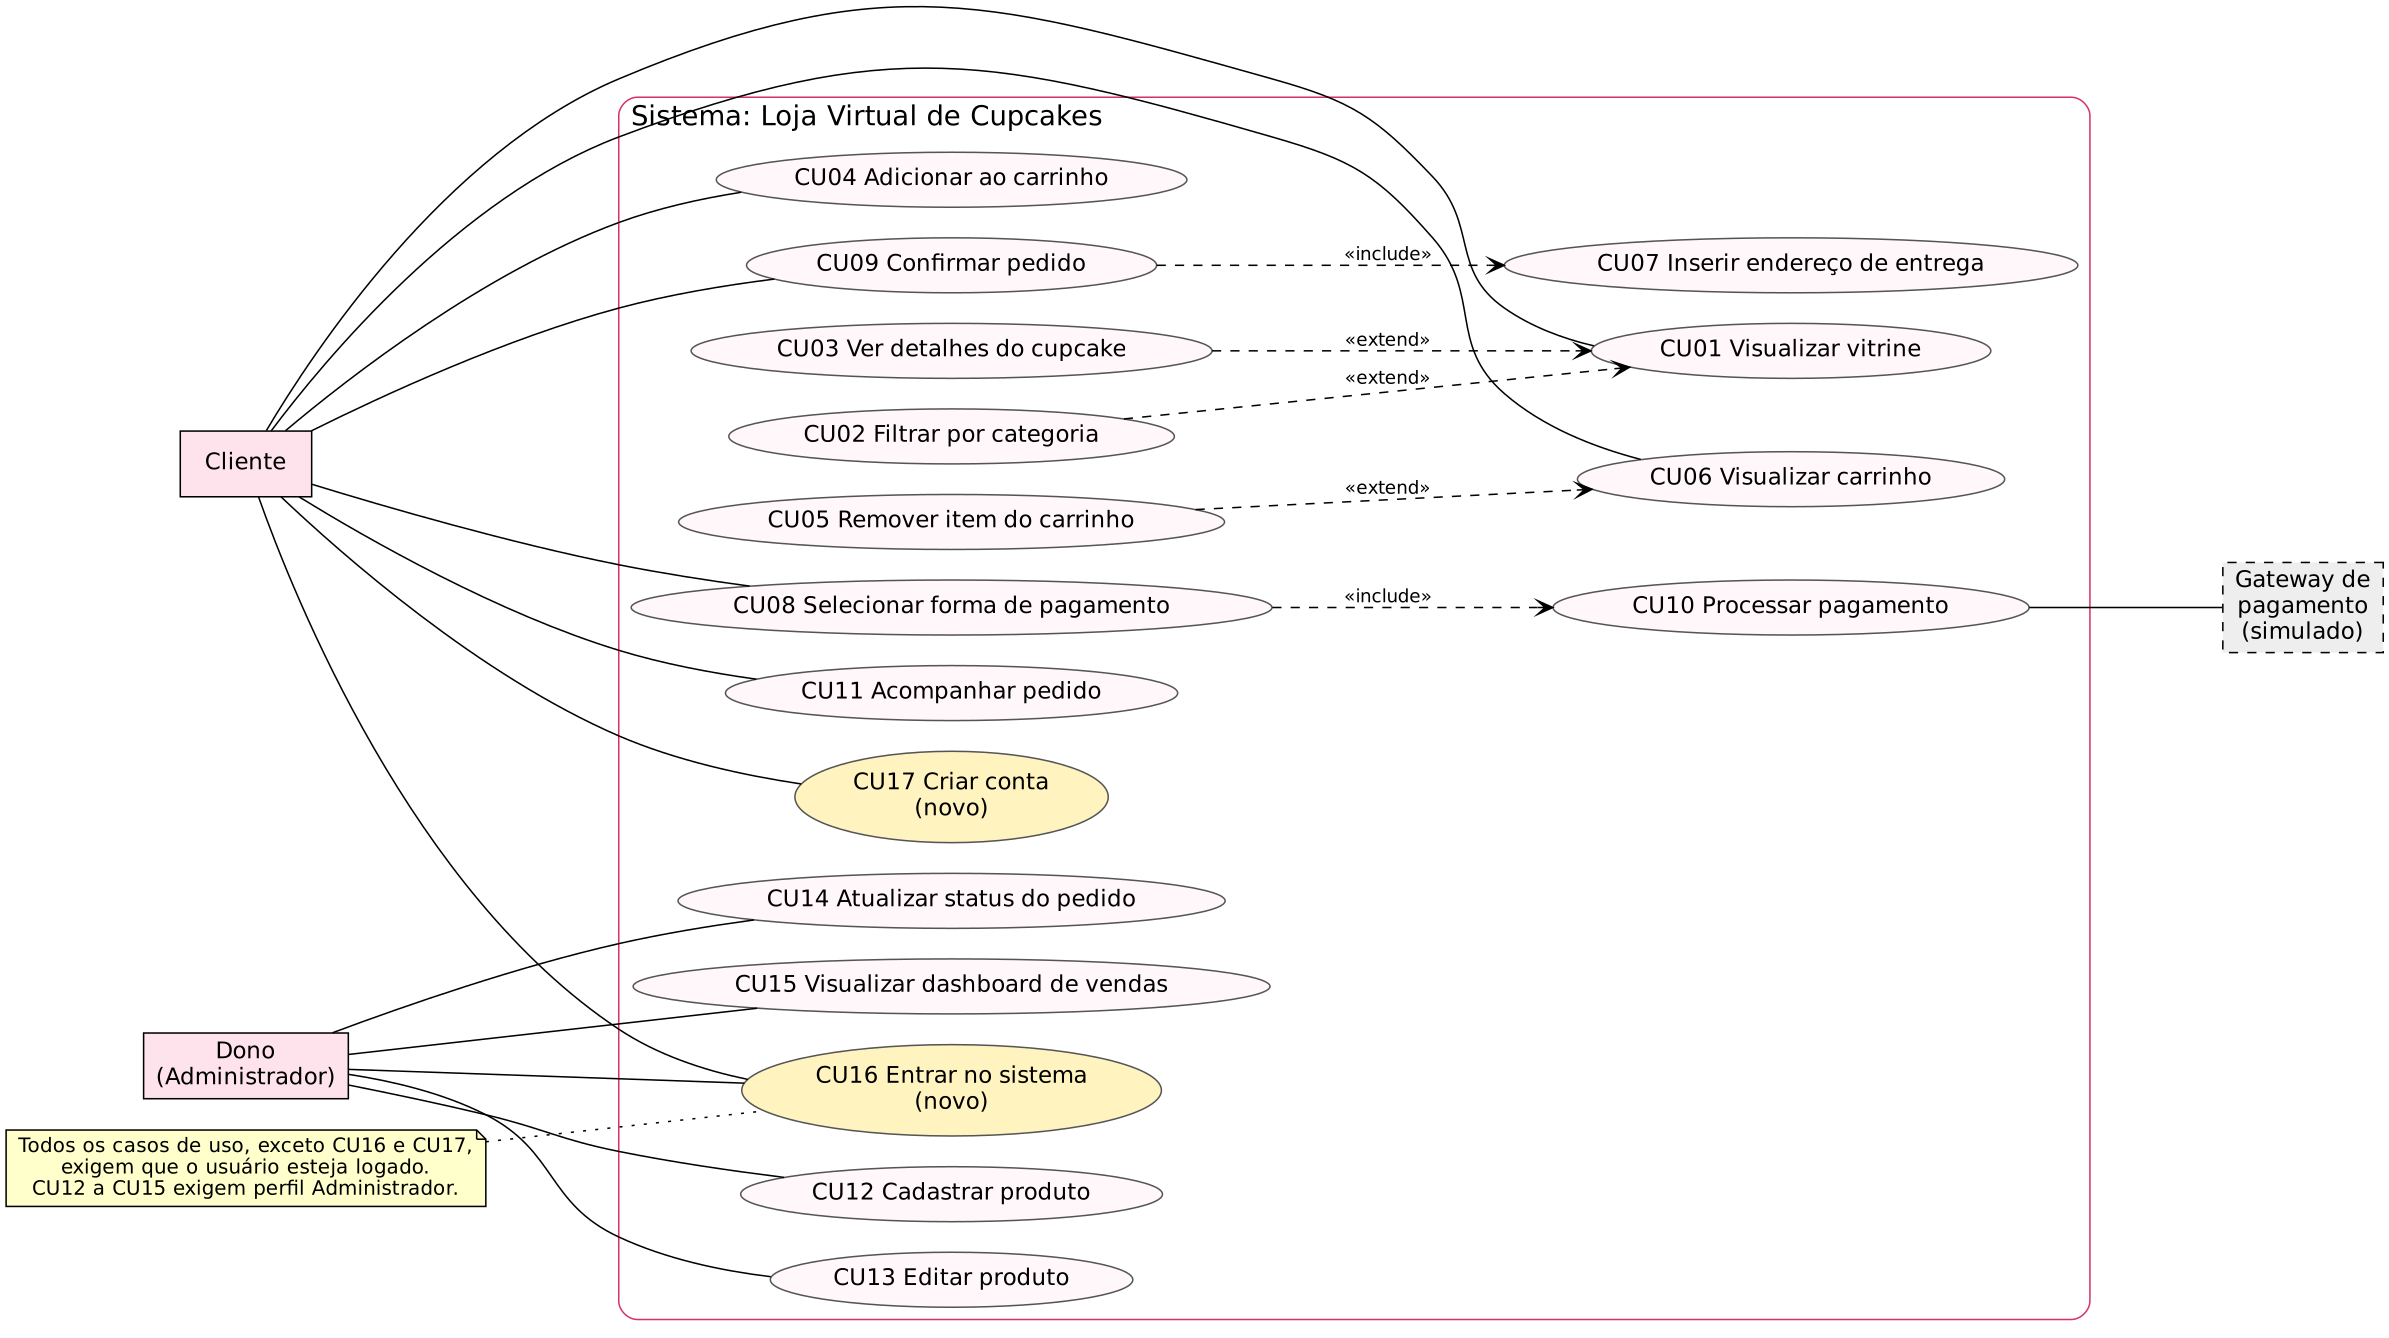
\includegraphics[width=0.93\linewidth, height=0.72\textheight, keepaspectratio]{img/casos_de_uso.png}
\caption{Diagrama de casos de uso revisado (em amarelo, os casos novos)}
\end{figure}
\end{landscape}

\textbf{Atores:} \textit{Cliente}, \textit{Dono} (administrador da loja) e \textit{Gateway de pagamento}, sistema externo (simulado nesta versão) que participa do CU10.

\textbf{Relações:} Filtrar por categoria (CU02) e Ver detalhes (CU03) estendem a vitrine (CU01). Remover item (CU05) estende a visualização do carrinho (CU06). Confirmar pedido (CU09) inclui a informação do endereço (CU07). Selecionar forma de pagamento (CU08) inclui o processamento do pagamento (CU10).

\subsection{Casos de uso novos e detalhados}

Os casos CU01 a CU10 do PITE I permanecem válidos. As alterações pontuais estão na seção~\ref{sec:ajustes}. A seguir, os casos que faltavam ou estavam incompletos.

\subsubsection{CU16 --- Entrar no sistema (novo)}
\textbf{Descrição:} identificar o usuário (cliente ou dono) para liberar as funções do seu perfil.\\
\textbf{Ator:} Cliente, Dono.\\
\textbf{Pré-condição:} usuário cadastrado e ativo.\\
\textbf{Pós-condição:} sessão aberta, tela correspondente ao perfil exibida.
\begin{enumerate}[nosep]
\item O sistema exibe somente a tela de login ao ser aberto;
\item O usuário informa e-mail e senha;
\item O sistema confere o e-mail e o \textit{hash} da senha; <Curso Alternativo Alfa>
\item O sistema cria a sessão e devolve um \textit{token};
\item Se o perfil for Cliente, o sistema exibe a vitrine; se for Administrador, exibe o painel do dono;
\item O caso de uso termina.
\end{enumerate}
\textbf{Alfa (credenciais inválidas):} Alfa3: e-mail ou senha não conferem ou o usuário está inativo; Alfa4: o sistema informa ``E-mail ou senha inválidos'' e permanece no login.

\subsubsection{CU17 --- Criar conta (novo)}
\textbf{Descrição:} permitir que um visitante se cadastre como cliente.\\
\textbf{Pré-condição:} o e-mail ainda não está cadastrado.\\
\textbf{Pós-condição:} cliente criado e apto a fazer login.
\begin{enumerate}[nosep]
\item O visitante abre a aba ``Criar conta'' e informa nome, e-mail, senha e, opcionalmente, telefone;
\item O sistema valida os campos: senha com ao menos 6 caracteres, telefone com 10 a 15 dígitos; <Curso Alternativo Alfa>
\item O sistema grava o usuário (perfil Cliente) e o cliente em uma única transação; <Curso Alternativo Beta>
\item O sistema informa que a conta foi criada e volta ao login com o e-mail preenchido;
\item O caso de uso termina.
\end{enumerate}
\textbf{Alfa (dados inválidos):} o sistema informa o problema e retorna ao passo 1.\\
\textbf{Beta (e-mail repetido):} o sistema informa ``E-mail já cadastrado'' e nada é gravado.

\subsubsection{CU11 --- Acompanhar pedido}
\textbf{Pré-condição:} cliente logado.\\
\textbf{Pós-condição:} o cliente vê o andamento de seus pedidos.
\begin{enumerate}[nosep]
\item O cliente abre a aba lateral ``Meus pedidos'';
\item O sistema consulta apenas os pedidos do cliente, do mais novo ao mais antigo (RN11);
\item O sistema exibe, para cada pedido, número, data, valor, status e situação do pagamento;
\item Para pedidos aguardando pagamento, o sistema oferece o botão ``Pagar agora'';
\item O sistema atualiza a lista a cada 15 segundos enquanto a aba estiver aberta;
\item O caso de uso termina.
\end{enumerate}
\textbf{Alfa (sem pedidos):} o sistema exibe ``Você ainda não fez pedidos''.

\subsubsection{CU12 --- Cadastrar produto}
\textbf{Ator:} Dono.\ \textbf{Pré-condição:} dono logado.\ \textbf{Pós-condição:} novo cupcake gravado.
\begin{enumerate}[nosep]
\item O dono abre o painel e preenche nome, descrição, preço, estoque, ingredientes, imagem, categorias, destaque e ativo;
\item O sistema valida os campos obrigatórios e o preço maior que zero (RN12); <Curso Alternativo Alfa>
\item O sistema grava o produto e suas categorias em uma única transação; <Curso Alternativo Beta>
\item O sistema informa ``Produto salvo'' e atualiza a lista de produtos e o dashboard;
\item O caso de uso termina.
\end{enumerate}
\textbf{Alfa (dados inválidos):} nome ou descrição vazios, preço zero ou negativo, estoque negativo: o sistema informa o erro e nada é gravado.\\
\textbf{Beta (nome repetido):} o sistema informa que já existe um produto com esse nome.

\subsubsection{CU13 --- Editar produto}
\textbf{Ator:} Dono.\ \textbf{Pré-condição:} produto existente.\ \textbf{Pós-condição:} dados atualizados; pedidos antigos continuam com o preço pago.
\begin{enumerate}[nosep]
\item O dono escolhe ``Editar'' em um produto e o formulário é preenchido com os dados atuais;
\item O dono altera preço, estoque, categorias, destaque ou o campo ``Ativo'';
\item O sistema valida (RN12) e confirma que o produto existe (RN13); <Curso Alternativo Alfa>
\item O sistema grava as alterações e recarrega a lista;
\item O caso de uso termina.
\end{enumerate}
\textbf{Alfa (produto inexistente):} o sistema informa ``Produto não encontrado''.\\
\textbf{Observação:} desmarcar ``Ativo'' retira o produto da vitrine sem apagá-lo; a reposição de estoque é feita informando o novo total.

\subsubsection{CU14 --- Atualizar status do pedido}
\textbf{Ator:} Dono.\ \textbf{Pré-condição:} pedido existente.\ \textbf{Pós-condição:} status alterado e registrado no histórico.
\begin{enumerate}[nosep]
\item O dono escolhe o novo status na lista do pedido;
\item O sistema verifica se a transição é permitida (RN14): aguardando pagamento $\rightarrow$ pago $\rightarrow$ em preparo $\rightarrow$ enviado $\rightarrow$ entregue, com cancelamento possível até o preparo; <Curso Alternativo Alfa>
\item O sistema grava o novo status e registra status anterior, novo status, responsável e data;
\item O sistema informa ``Status atualizado'' e recarrega pedidos e dashboard;
\item O caso de uso termina.
\end{enumerate}
\textbf{Alfa (transição inválida):} o sistema informa ``Transição de status inválida'' e mantém o status anterior.

\subsubsection{CU15 --- Visualizar dashboard de vendas}
\textbf{Ator:} Dono.\ \textbf{Pré-condição:} dono logado.\ \textbf{Pós-condição:} indicadores exibidos com dados atuais (RN15).
\begin{enumerate}[nosep]
\item O dono abre o painel;
\item O sistema consulta as vendas por dia (pedidos pagos, faturamento e ticket médio), os produtos mais vendidos e a situação do estoque;
\item O sistema exibe as três tabelas; pedidos aguardando pagamento ou cancelados não entram nas vendas;
\item O caso de uso termina.
\end{enumerate}
\textbf{Alfa (sem vendas):} o sistema exibe ``Sem dados''.

\subsection{Ajustes nos casos de uso existentes}
\label{sec:ajustes}

\begin{table}[H]
\centering\small\renewcommand{\arraystretch}{1.3}
\begin{tabular}{|c|p{12cm}|}
\hline
\rowcolor{gray!30} \textbf{Caso} & \textbf{Ajuste} \\ \hline
CU01 & A vitrine só é exibida depois do login (CU16). \\ \hline
CU04 & Cada clique em ``Adicionar'' soma uma unidade; a quantidade final é ajustada clicando novamente. A faixa válida é de 1 a 99 (RN04). \\ \hline
CU05 & O item é removido por inteiro, sem etapa de confirmação (a confirmação prevista no PITE I não foi implementada). \\ \hline
CU07 & O endereço é escolhido, ou cadastrado, na janela de finalização do pedido. Os dados são validados no servidor (CEP com 8 dígitos, UF com 2 letras). \\ \hline
CU08 e CU10 & A forma de pagamento é escolhida na janela de pagamento, aberta depois da confirmação do pedido. Um pagamento recusado permite nova tentativa. O gateway é simulado. \\ \hline
CU09 & A confirmação grava os itens com o preço do momento, copia o endereço, baixa o estoque e fecha o carrinho em uma única transação. \\ \hline
\end{tabular}
\caption{Ajustes aos casos de uso do PITE I}
\end{table}

% ================================================================= 3
\section{Diagrama de classes revisado}

\begin{figure}[H]
\centering
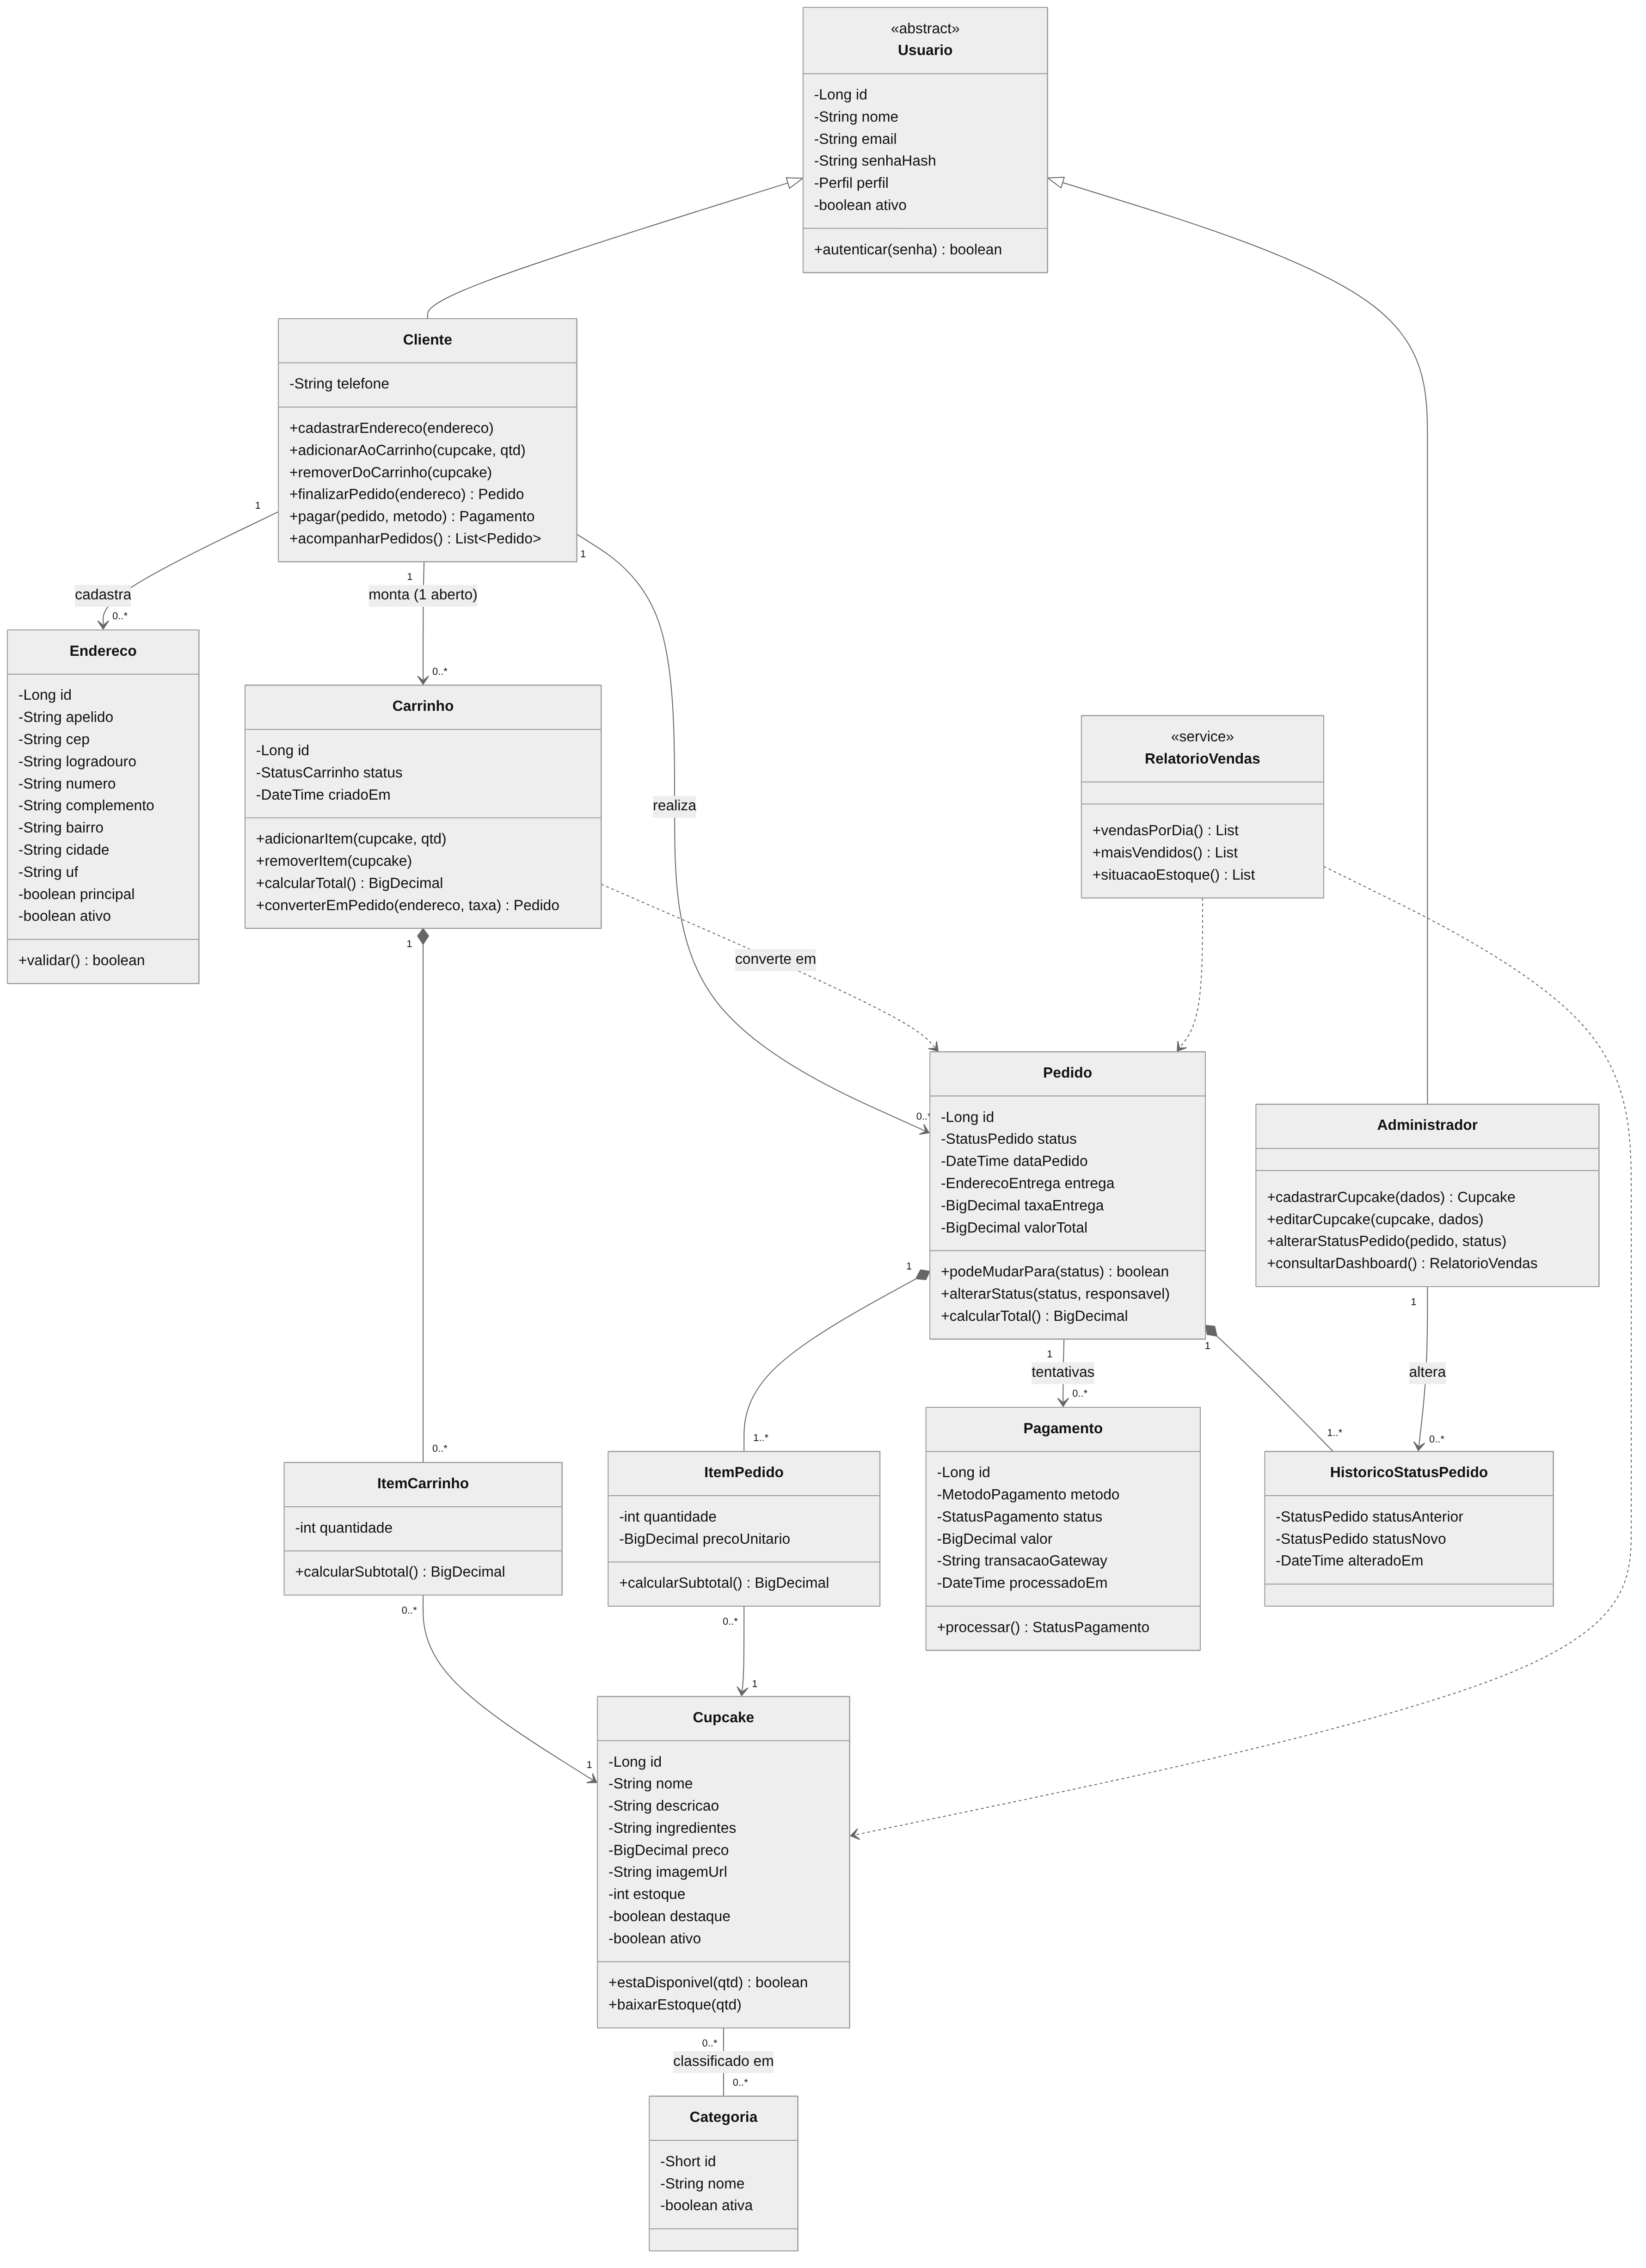
\includegraphics[width=\textwidth, height=0.86\textheight, keepaspectratio]{img/classes.png}
\caption{Diagrama de classes de domínio revisado}
\end{figure}

\subsection{Dicionário das classes}

\begin{table}[H]
\centering\small\renewcommand{\arraystretch}{1.3}
\begin{tabular}{|p{3.4cm}|p{10.4cm}|}
\hline
\rowcolor{gray!30} \textbf{Classe} & \textbf{Responsabilidade} \\ \hline
Usuario (abstrata) & Credenciais e perfil de quem acessa o sistema. Senha guardada apenas como \textit{hash} \\ \hline
Cliente & Usuário que compra: mantém endereços, carrinho e pedidos \\ \hline
Administrador & Dono da loja: gerencia produtos e pedidos e consulta as vendas \\ \hline
Endereco & Endereço de entrega salvo pelo cliente (valida CEP e UF) \\ \hline
Categoria & Rótulo de classificação (Chocolate, Vegano, Sem lactose etc.) \\ \hline
Cupcake & Produto à venda, com preço, estoque, destaque e indicador ativo \\ \hline
Carrinho / ItemCarrinho & Compras em andamento; um cliente tem no máximo um carrinho aberto \\ \hline
Pedido / ItemPedido & Compra confirmada; guarda o preço de cada item e uma cópia do endereço de entrega \\ \hline
Pagamento & Cada tentativa de pagamento do pedido, com método, status e código do gateway \\ \hline
HistoricoStatusPedido & Registro de cada mudança de status, com o responsável \\ \hline
RelatorioVendas (serviço) & Consultas do dashboard: vendas por dia, mais vendidos e situação do estoque \\ \hline
\end{tabular}
\caption{Classes do domínio}
\end{table}

\subsection{Enumerações}

\begin{table}[H]
\centering\small\renewcommand{\arraystretch}{1.3}
\begin{tabular}{|l|p{9.6cm}|}
\hline
\rowcolor{gray!30} \textbf{Enumeração} & \textbf{Valores} \\ \hline
Perfil & CLIENTE, ADMINISTRADOR \\ \hline
StatusCarrinho & ABERTO, CONVERTIDO, ABANDONADO \\ \hline
StatusPedido & AGUARDANDO\_PAGAMENTO, PAGO, EM\_PREPARO, ENVIADO, ENTREGUE, CANCELADO \\ \hline
MetodoPagamento & PIX, CARTAO \\ \hline
StatusPagamento & PENDENTE, APROVADO, RECUSADO, ESTORNADO \\ \hline
\end{tabular}
\caption{Enumerações usadas pelas classes}
\end{table}

\subsection{Decisões de modelagem}

\begin{itemize}
\item \textbf{Pedido e Pagamento (1 para N):} o fluxo alternativo do CU10 devolve o cliente à escolha de pagamento, o que gera mais de uma tentativa para o mesmo pedido.
\item \textbf{Cupcake e Categoria (N para N):} um cupcake vegano de chocolate precisa aparecer nos dois filtros (US02).
\item \textbf{ItemPedido guarda o preço:} alterar o preço de um cupcake não pode mudar pedidos já feitos.
\item \textbf{Endereço de entrega copiado no pedido:} o cliente pode editar seus endereços sem alterar o histórico de entregas.
\item \textbf{Relatório como serviço:} os relatórios são consultas calculadas sobre pedidos e produtos; não têm identidade própria nem são gravados.
\item \textbf{Valores monetários em BigDecimal:} evita erros de arredondamento do tipo \textit{double}.
\end{itemize}

% ================================================================= 4
\section{Diagramas de sequência}

Os quatro diagramas mostram o fluxo normal e os fluxos de erro dos principais casos de uso. Os nomes das mensagens seguem o código: tela (View), \textit{controllers}, DAOs e banco.

\subsection{Entrar no sistema e ver a vitrine (CU16, CU01)}
\figura{seq1.png}{Sequência: entrar e exibir a vitrine}{1.0}

\subsection{Adicionar ao carrinho (CU04, CU06)}
\figura{seq2.png}{Sequência: adicionar ao carrinho}{1.0}

\begin{landscape}
\subsection{Finalizar o pedido e pagar (CU07 a CU10)}
\begin{figure}[H]
\centering
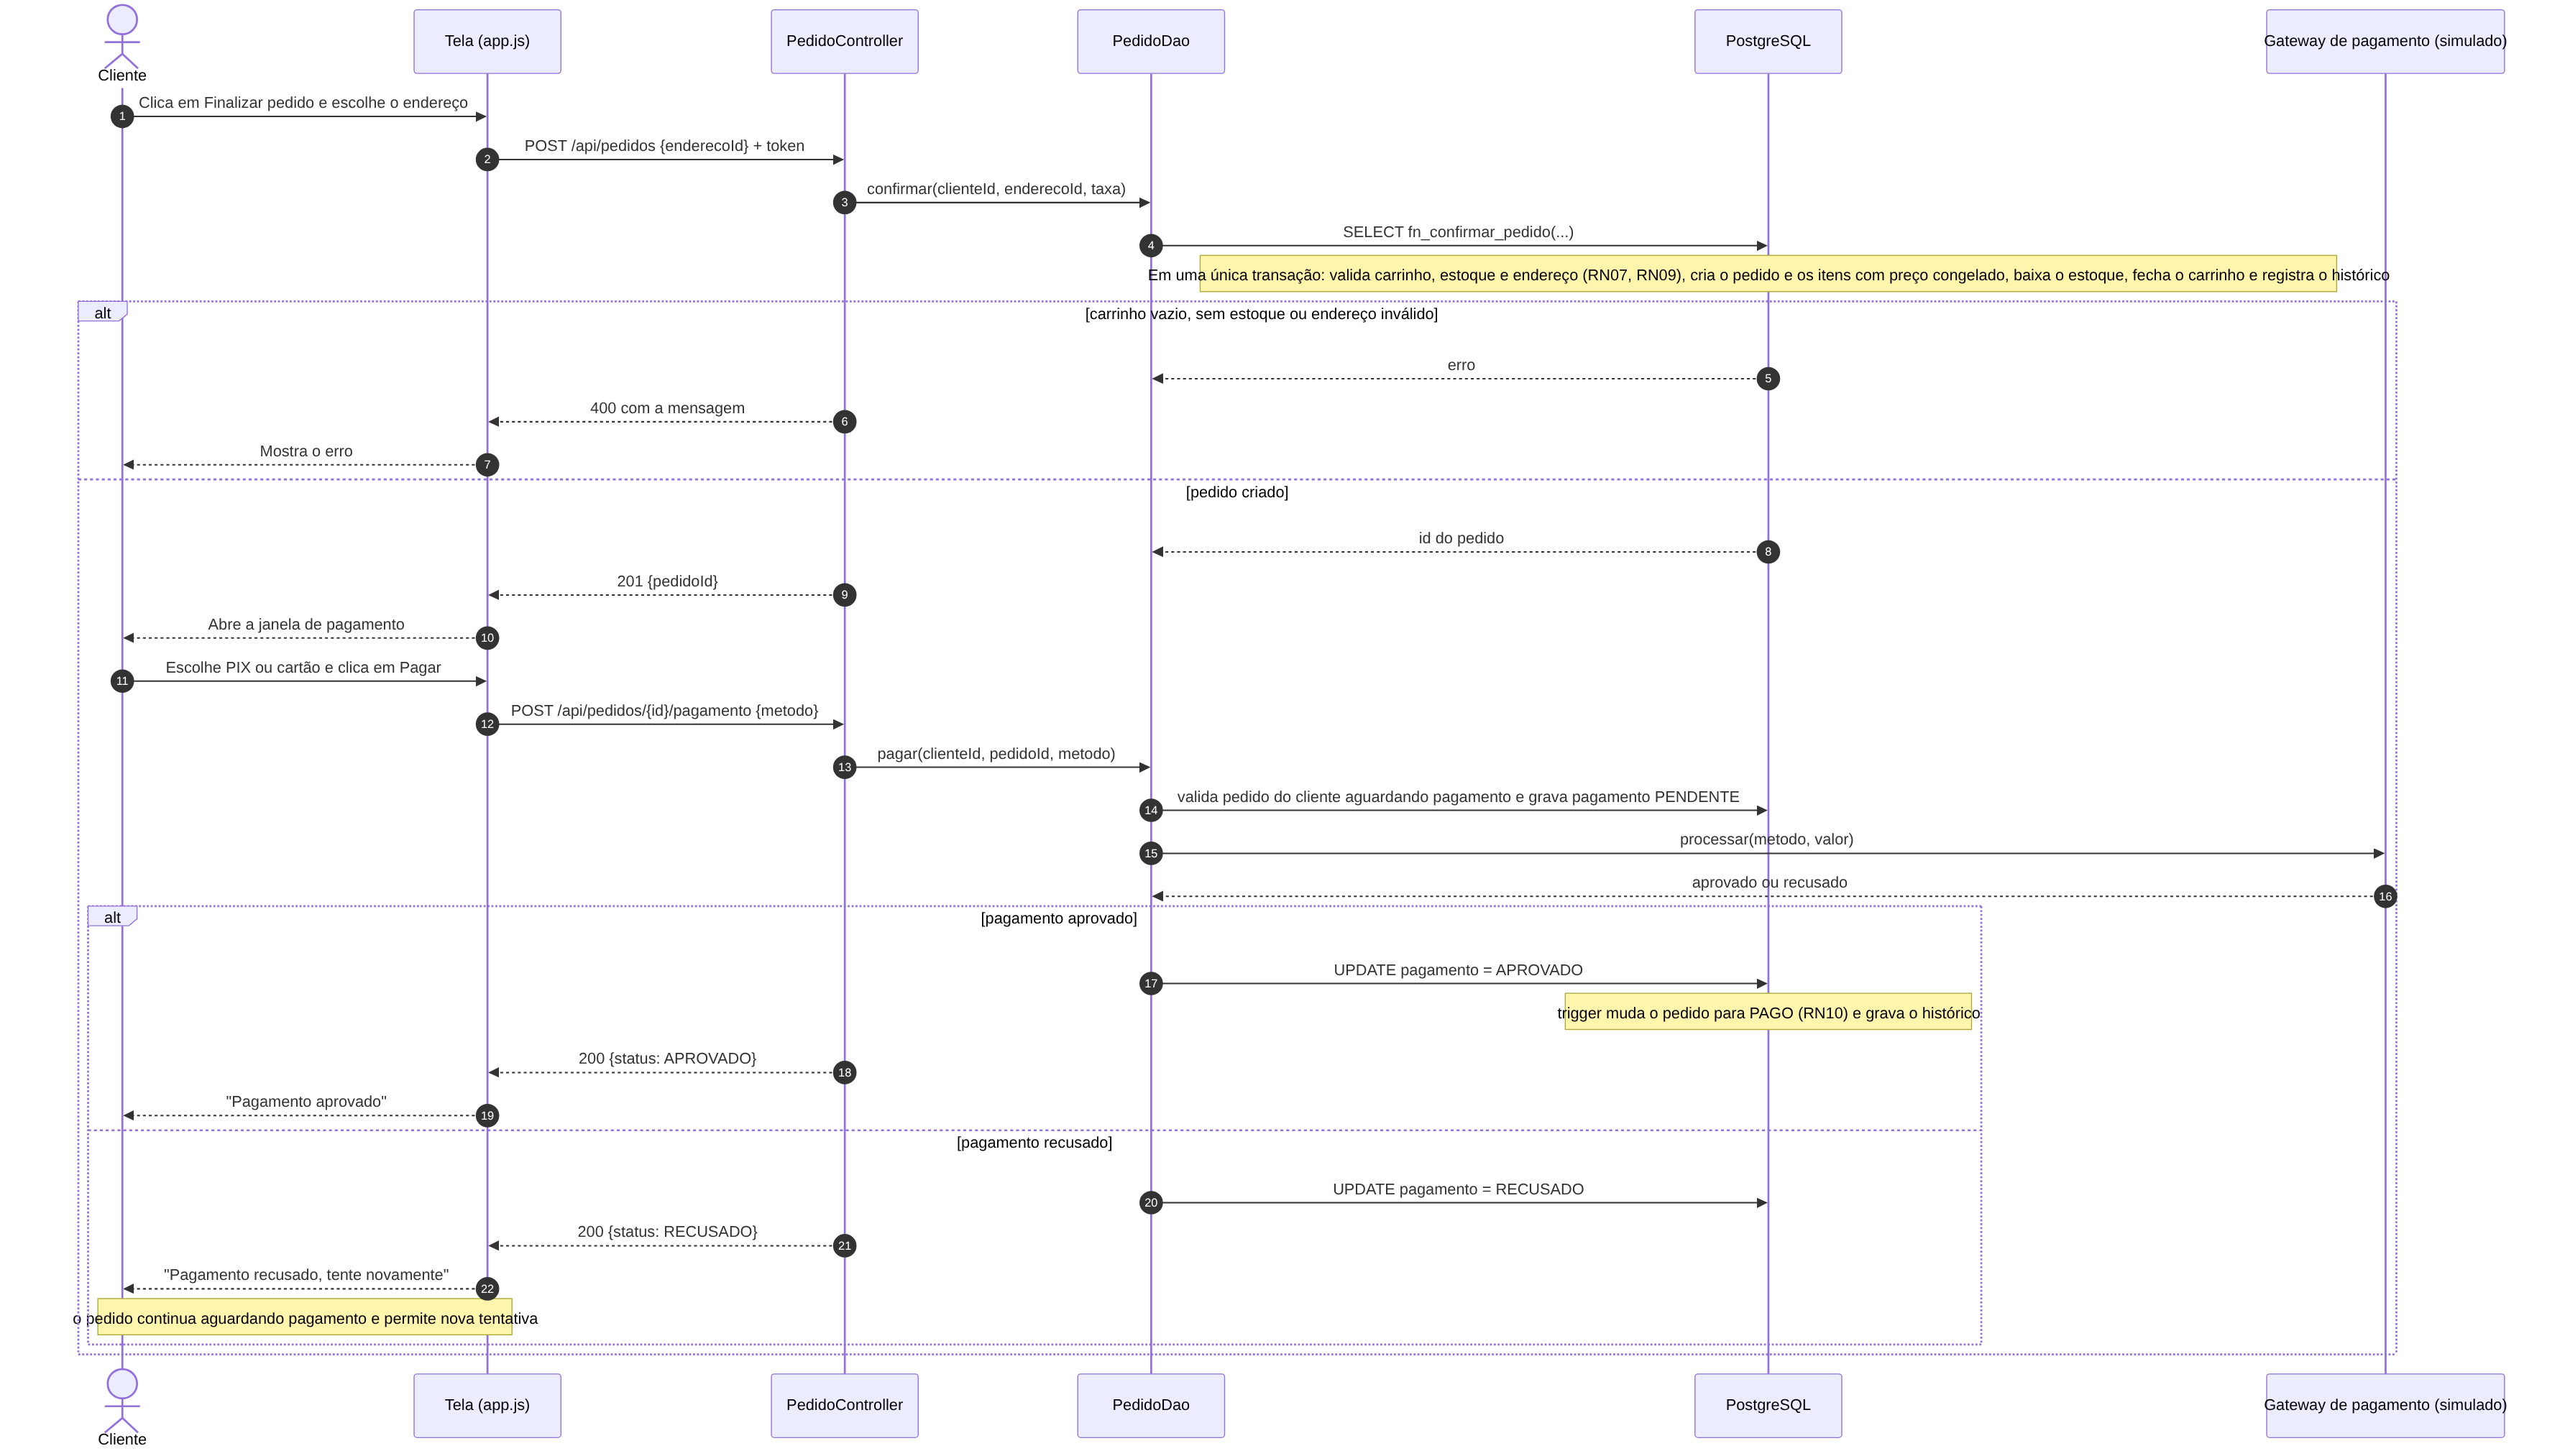
\includegraphics[width=0.95\linewidth, height=0.7\textheight, keepaspectratio]{img/seq3.png}
\caption{Sequência: finalizar o pedido e pagar}
\end{figure}
\end{landscape}

\subsection{Dono atualiza o status do pedido (CU14)}
\figura{seq4.png}{Sequência: atualização de status pelo dono}{1.0}

% ================================================================= 5
\section{Arquitetura em camadas}

\figura{camadas.png}{Camadas do sistema (MVC) e acesso ao banco}{1.0}

A \textit{View} é composta pelas páginas e scripts da pasta \texttt{public}. Os \textit{Controllers} recebem as requisições da API, validam o formato dos dados e escolhem a resposta. O \textit{Model} reúne os registros e os DAOs, únicos pontos que falam com o PostgreSQL. As regras de negócio mais sensíveis ficam no próprio banco (restrições, \textit{triggers} e a função que confirma o pedido).

% ================================================================= 6
\section{Projeto conceitual de dados}
\label{sec:conceitual}

O modelo conceitual descreve o que precisa ser guardado, independentemente de tecnologia: entidades, atributos, identificadores, relacionamentos e cardinalidades. Foi derivado do diagrama de classes revisado e dá origem ao modelo lógico normalizado e ao projeto físico, apresentados no documento do banco de dados.

\subsection{Diagrama entidade-relacionamento conceitual}

\begin{figure}[H]
\centering
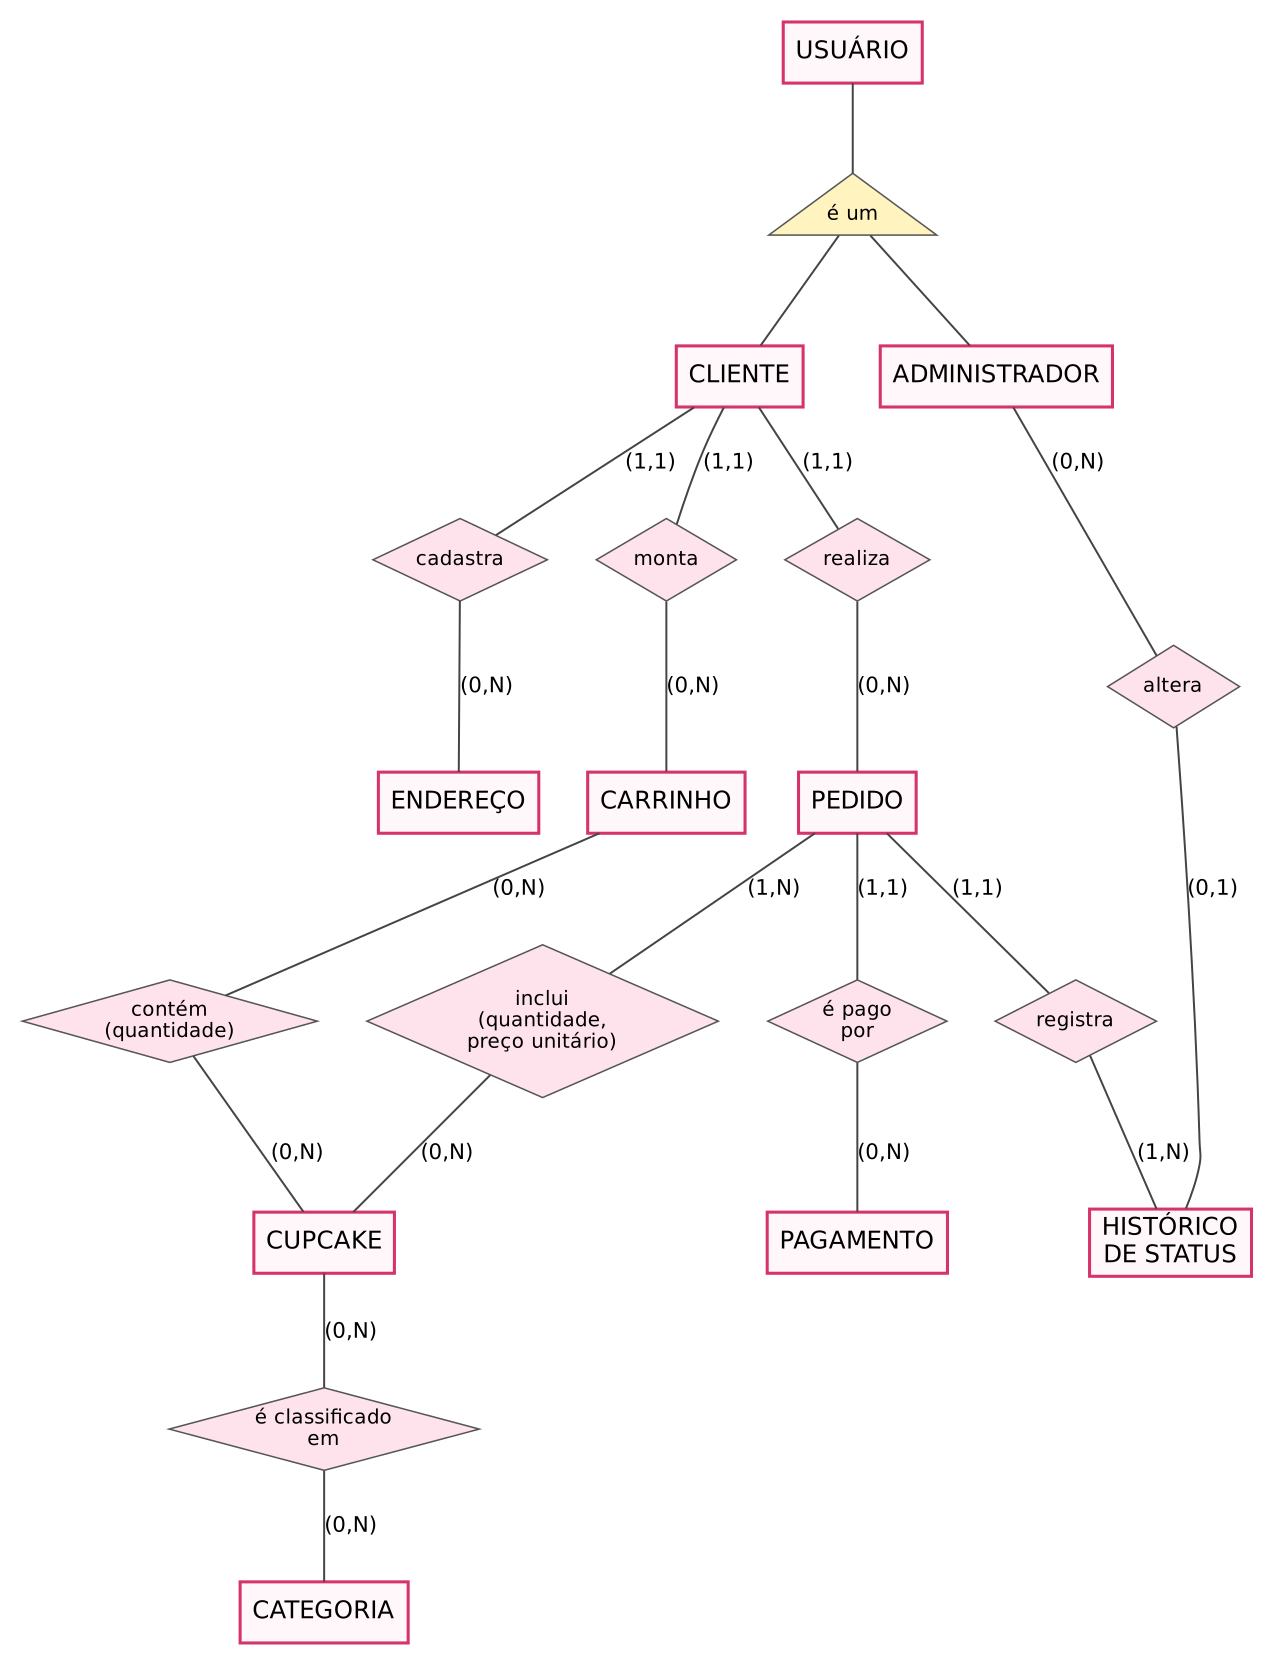
\includegraphics[width=\textwidth, height=0.8\textheight, keepaspectratio]{img/der_conceitual.png}
\caption{Modelo conceitual de dados: entidades, relacionamentos e cardinalidades na notação (mínimo, máximo). Os atributos de cada entidade estão na tabela da seção~\ref{sec:atributos}}
\end{figure}

\subsection{Entidades e atributos}
\label{sec:atributos}

\begin{longtable}{|p{3.0cm}|p{6.4cm}|p{4.2cm}|}
\hline
\rowcolor{gray!30} \textbf{Entidade} & \textbf{Atributos} & \textbf{Identificador} \\ \hline
\endhead
Usuário & nome, e-mail, senha, perfil, ativo & código (e-mail é único) \\ \hline
Cliente & telefone & herda o código do usuário \\ \hline
Administrador & (nenhum próprio) & herda o código do usuário \\ \hline
Endereço & apelido, CEP, logradouro, número, complemento, bairro, cidade, UF, principal & código \\ \hline
Categoria & nome, ativa & código (nome é único) \\ \hline
Cupcake & nome, descrição, ingredientes, preço, imagem, estoque, destaque, ativo & código (nome é único) \\ \hline
Carrinho & status, data de criação & código \\ \hline
Pedido & data, status, endereço de entrega (cópia), taxa de entrega, valor total & número \\ \hline
Pagamento & método, status, valor, código da transação, data de processamento & código \\ \hline
Histórico de status & status anterior, status novo, data da alteração & código \\ \hline
\end{longtable}

\subsection{Relacionamentos e cardinalidades}

\small
\begin{longtable}{|p{3.1cm}|p{3.6cm}|p{2.5cm}|p{4.4cm}|}
\hline
\rowcolor{gray!30} \textbf{Relacionamento} & \textbf{Entidades} & \textbf{Cardinalidade} & \textbf{Leitura} \\ \hline
\endhead
é um & Usuário, Cliente, Administrador & especialização & Todo usuário é cliente ou administrador \\ \hline
cadastra & Cliente (1,1) e Endereço (0,N) & 1:N & Um cliente cadastra vários endereços; cada endereço pertence a um cliente \\ \hline
monta & Cliente (1,1) e Carrinho (0,N) & 1:N & Um cliente monta vários carrinhos ao longo do tempo (um aberto por vez) \\ \hline
realiza & Cliente (1,1) e Pedido (0,N) & 1:N & Um cliente realiza vários pedidos \\ \hline
contém & Carrinho (0,N) e Cupcake (0,N) & N:N, com quantidade & Um carrinho tem vários cupcakes e um cupcake está em vários carrinhos \\ \hline
é classificado em & Cupcake (0,N) e Categoria (0,N) & N:N & Um cupcake tem várias categorias e uma categoria agrupa vários cupcakes \\ \hline
inclui & Pedido (1,N) e Cupcake (0,N) & N:N, com quantidade e preço unitário & Um pedido inclui ao menos um cupcake; o preço fica gravado \\ \hline
é pago por & Pedido (1,1) e Pagamento (0,N) & 1:N & Um pedido pode ter várias tentativas de pagamento \\ \hline
registra & Pedido (1,1) e Histórico (1,N) & 1:N & Todo pedido tem ao menos um registro de status (o inicial) \\ \hline
altera & Administrador (0,N) e Histórico (0,1) & 1:N & Uma alteração feita pelo dono guarda o responsável; a mudança automática por pagamento não tem responsável \\ \hline
\end{longtable}

\normalsize
\subsection{Regras de integridade do modelo}

\begin{itemize}
\item Um cliente tem no máximo um carrinho aberto e no máximo um endereço principal ativo.
\item Um pedido tem no máximo um pagamento aprovado.
\item Quantidades dos itens são sempre maiores ou iguais a 1; preço e estoque nunca são negativos.
\item O status do pedido só muda segundo o fluxo permitido (RN14), e cada mudança é registrada.
\item Cupcakes e pedidos não são apagados: produtos saem da vitrine ao serem desativados, e pedidos guardam seus itens e preços.
\item Pedidos e pagamentos não podem ser excluídos pela aplicação.
\end{itemize}

\subsection{Do conceitual ao lógico}

\begin{table}[H]
\centering\small\renewcommand{\arraystretch}{1.3}
\begin{tabular}{|p{4.6cm}|p{9.2cm}|}
\hline
\rowcolor{gray!30} \textbf{No modelo conceitual} & \textbf{No modelo lógico (tabelas)} \\ \hline
Especialização Usuário, Cliente e Administrador & Tabela \texttt{usuario} com o campo \texttt{perfil}; tabela \texttt{cliente} com a chave igual à de \texttt{usuario} \\ \hline
Relacionamentos 1:N & Chave estrangeira no lado ``N'' (por exemplo, \texttt{endereco.cliente\_id}) \\ \hline
Relacionamentos N:N (contém, inclui, é classificado em) & Tabelas associativas \texttt{item\_carrinho}, \texttt{item\_pedido} e \texttt{cupcake\_categoria}, com chave composta \\ \hline
Atributos dos relacionamentos (quantidade, preço unitário) & Colunas das tabelas associativas \\ \hline
Endereço de entrega (cópia) no pedido & Colunas \texttt{entrega\_*} na tabela \texttt{pedido} \\ \hline
Relatório & \textit{Views} (\texttt{vw\_vendas\_diarias}, \texttt{vw\_produtos\_mais\_vendidos}, \texttt{vw\_estoque}) \\ \hline
\end{tabular}
\caption{Transformação do modelo conceitual em lógico}
\end{table}

\end{document}
